\chapter{Graph Isomorphism, Subgraph Isomorphism}

Rishnak was frantically looking for Ajur as he wanted to share with him some important concepts. Finally he found Ajur and Jura walking along the bank of a pond in the cemetery. Rishnak told Ajur that we have been talking about Graphs and some times, we label the vertices and sometimes we do not label the vertices. Rishnak told Ajur that the graph with vertices labeled is called a labeled graph and the one without labels is called an unlabeled graph. Two labeled graphs are equivalent if they are identical- all the edges have the same labels. Here are two labeled graphs that are equivalent see Figures \ref{8g1} and \ref{8g11}. Graph see Figure \ref{8g2} is not equivalent to either Graph \ref{8g1} or \ref{8g11} ad in Graph \ref{8g2} there is no edge between vertices 4 and 5.
\begin{figure}
\begin{center}
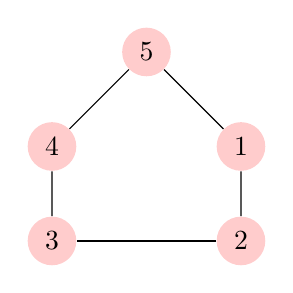
\begin{tikzpicture}
  [scale=.6,auto=left,every node/.style={circle,fill=red!20}]
  \node (n1) at (5,5) {1};
  \node (n4) at (1,5)  {4};
  \node (n3) at  (1,3) {3};
  \node (n2) at (5,3)  {2};
  \node (n5) at (3,7)  {5};

  \foreach \from/\to in {n1/n2,n2/n3,n3/n4,n4/n5,n1/n5}
    \draw (\from) -- (\to);

\end{tikzpicture}
\caption{Labeled Graph}\label{8g1}
\end{center}

\end{figure}
\begin{figure}
\begin{center}
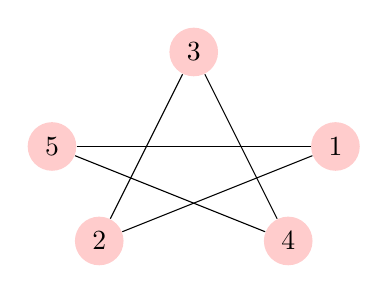
\begin{tikzpicture}
  [scale=.6,auto=left,every node/.style={circle,fill=red!20}]
   \node (n1) at (6,5) {1};
  \node (n5) at (0,5)  {5};
  \node (n2) at  (1,3) {2};
  \node (n4) at (5,3)  {4};
  \node (n3) at (3,7)  {3};

  \foreach \from/\to in {n1/n2,n2/n3,n3/n4,n4/n5,n5/n1}
    \draw (\from) -- (\to);

\end{tikzpicture}
\caption{ Another labeled graph with five vertices equivalent to Figure \ref{8g1}}\label{8g11}
\end{center}
\end{figure}

\begin{figure}
\begin{center}
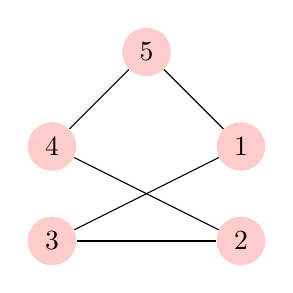
\begin{tikzpicture}
  [scale=.6,auto=left,every node/.style={circle,fill=red!20}]
   \node (n1) at (5,5) {1};
  \node (n4) at (1,5)  {4};
  \node (n3) at  (1,3) {3};
  \node (n2) at (5,3)  {2};
  \node (n5) at (3,7)  {5};


  \foreach \from/\to in {n1/n3,n2/n4,n3/n2,n1/n5,n5/n4}
    \draw (\from) -- (\to);

\end{tikzpicture}
\caption{ Another labeled graph with five vertices which is not equivalent to Graphs \ref{8g1} and \ref{8g11} as the edge labels are distinct from either of the two graphs}\label{8g2}
\end{center}
\end{figure}

Two graphs are isomorphic (structurally the same), if they are equivalent under vertex relabeling. So if in Graph \ref{8g2} vertex 2 is relabeled as 3 and vertex 3 is relabeled as 2, the two graphs \ref{8g2} and \ref{8g1} are equivalent. If a graph, $G$, is equivalent to a graph $H$ and $H$ is equivalent to another graph $P$, then $G$ is equivalent to graph $P$\footnote{Equivalence relation is transitive.}. To test whether two graphs are isomorphic are not is a hard\footnote{Not as hard as finding a Hamiltonian Cycle in a graph} problem.

If two graphs are isomorphic, they should have the same number of vertices, same number of edges, same degree sequences, length of the longest cycle, length of the shortest cycle and many more properties.  These properties of graphs are called invariant of graphs. By no mean these invariants are exhaustive. We do not know of a single invariant (that could be easily computed) that can be used to test whether or not two given graphs are isomorphic. 

Rishnak asked Ajur, can you provide two graphs which have the same number of vertices and same number of edges but they are not isomorphic. Ajur thought a bit, and he was able to produce the following two graphs which have 6 vertices and 9 edges. Ajur added that one graph is bipartite (all cycles are of even length) \ref{8g3} and the other one is not bipartite (cycle of length 3) \ref{8g4} and hence these two graphs are not isomorphic.

\begin{figure}

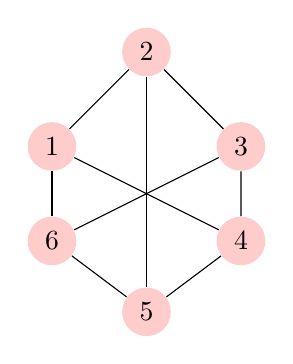
\begin{tikzpicture}
  [scale=.3,auto=left,every node/.style={circle,fill=red!20}]
  \node (n1) at (1,7) {1};
  \node (n2) at (5,11)  {2};
  \node (n3) at (9,7)  {3};
  \node (n4) at (9,3) {4};
  \node (n5) at (5,0)  {5};
  \node (n6) at (1,3) {6};
  
   \foreach \from/\to in {n1/n2,n2/n3,n3/n4,n4/n5,n5/n6,n1/n6,
  n2/n5, n6/n3,n1/n4}
    \draw (\from) -- (\to);
    \end{tikzpicture}
\caption{ A Bipartite Graph with 6 vertices and 9 edges same as Graph in \ref{5g5}}\label{8g3}

\end{figure}

\begin{figure}

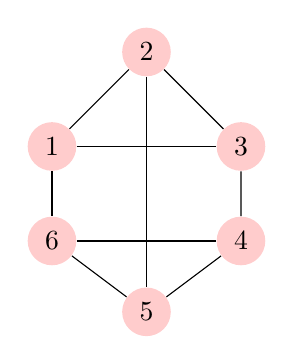
\begin{tikzpicture}
  [scale=.3,auto=left,every node/.style={circle,fill=red!20}]
  \node (n1) at (1,7) {1};
  \node (n2) at (5,11)  {2};
  \node (n3) at (9,7)  {3};
  \node (n4) at (9,3) {4};
  \node (n5) at (5,0)  {5};
  \node (n6) at (1,3) {6};
  
   \foreach \from/\to in {n1/n2,n2/n3,n3/n4,n4/n5,n5/n6,n1/n6,
  n2/n5, n6/n4,n1/n3}
    \draw (\from) -- (\to);
    \end{tikzpicture}
\caption{ A nonbipartite Graph with 6 vertices and 9 edges}\label{8g4}

\end{figure}

Ajur thought for a while and said these isomorphism problems will be very useful when you want to test whether a given graph is in a collection of graphs - a very useful tool may be for Chemists. Rishnak was happy to see Ajur's thinking and finding practical uses for isomorphism problem. 

Ajur asked Rishnak is there an easier method for testing isomorphism between rooted trees. Rishnak smiled and said there is a faster method for rooted trees. Before that Rishnak wanted to explain a canonical representation for a labeled tree. One such canonical representation is a Pr{\"u}fer code. Rishnak explained how to get a code of length $n-2$ for a labeled tree (with consecutive positive integers) with  $n$ vertices.

\begin{enumerate}
\item let Pr{\"u}fer code be an empty set,

\item Start with a leaf vertex (leaf vertex is a vertex of degree 1) of lowest label say v. Find the vertex connecting it to the rest of tree say w.  Remove v from the tree and add w to the Pr{\"u}fer Code
 
\item Repeat the previous step until we are left with two vertices.
\end{enumerate}

For example the Pr{\"u}fer code for the following tree is: The smallest leaf vertex is 4. Its adjacent vertex is labeled 2. So 2 is added to the Pr{\"u}fer code and vertex 4 is removed. Next smallest vertex is 5 and its adjacent vertex is 2. Hence 2 is added to the Pr{\"u}fer code and vertex labeled 5 is removed. Now 2 is the smallest leaf vertex and its adjacent vertex is 1 and  1 is added to Pr{\"u}fer code and vertex 2 is removed. Currently Pr{\"u}fer code is \textbf{221}. Now 1 is the smallest labeled vertex and its adjacent vertex is 3 and vertex 1 is removed. Hence 3 is added to Pr{\"u}fer code which becomes \textbf{2213}. The next smallest leaf vertex is 6 and its adjacent vertex is 3. 3 is added to Pr{\"u}fer code. There are only two vertices left and we are done. Pr{\"u}fer code for tree \ref{8g5} is \textbf{22133}. From this Pr{\"u}fer code, one can conclude that there are 7 vertices in the tree (as the Pr{\"u}fer code is of length $n-2$ for a tree with $n$ vertices). Further, we can also conclude that vertices labeled 4,5,6 and 7 are leaf vertices as they do not appear in the given Pr{\'u}fer code. 
\begin{figure}
\begin{center}

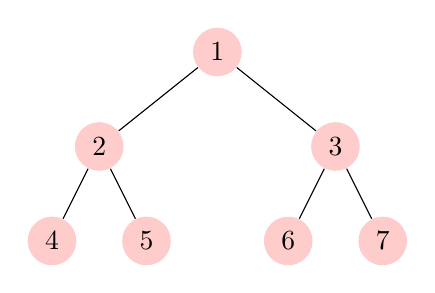
\begin{tikzpicture}
  [scale=.6,auto=left,every node/.style={circle,fill=red!20}]
  \node (n1) at (5.5,7) {1};
  \node (n2) at (3,5)  {2};
  \node (n3) at (8,5)  {3};
  \node (n4) at (2,3) {4};
  \node (n5) at (4,3)  {5};
  \node (n6) at (7,3)  {6};
  \node (n7) at (9,3)  {7};

  \foreach \from/\to in {n1/n2,n1/n3,n2/n4,n2/n5,n3/n6,n3/n7}
    \draw (\from) -- (\to);

\end{tikzpicture}

\caption{Tree with 7 vertices and four leaf vertices at the ground. }\label{8g5}
\end{center}
\end{figure}

Ajur asked Rishnak whether we can have a code for unlabeled trees. Rishnak replied with a resounding yes. Rishnak explained the basic steps for a rooted tree. For any tree, you need to choose an appropriate root vertex \footnote{Center of a tree is chosen as the root vertex} 
\begin{enumerate}
    \item  Label the leaf vertices as 01.
    \item If all the children of a vertex, $x$ have labels, sort these labels in alphabetical order footnote{0 comes before 1} The label of vertex $x$is 0 followed by concatenation of these sorted vertices followed by 1.
    \item Stop after you label the root vertex.
\end{enumerate}

For example for the tree in \ref{8g5} leaf vertices 4,5,6,7 are all labeled \textbf{01}. Vertex 2 is labeled \textbf{001011} and vertex 3 has a similar label \textbf{001011}. Finally root vertex has the label \textbf{00101100101111}. This \textbf{00101100101111} becomes the code for the tree.

Rishnak said that there is a closely related problem to Graph Isomorphism problem which has plenty of uses in real life - and not just in ghostly life. Ajur chuckled at the bad joke of Rishnak but did not want to interrupt him. Rishnak continued that instead of asking whether two graphs are structurally similar, given two graphs $G$ and $H$, subgraph isomorphism problem asks if there is a subgraph of $G$ that is isomorphic to H. Ajur immediately said then we can use this to test whether a graph $G$ with $n$ vertices has a Hamiltonian cycle by choosing $H$ to be a cycle of length $n$ and asking whether there is a subgraph of $G$ isomorphic to $H$. Rishnak agreed to what Ajur pointed and said that is why subgraph Isomorphism problem is very hard. On the other hand, if both $G$ and $H$ are labeled graphs, there are heuristics to test whether $H$ occurs in $G$ as a subgraph. This kind of labeled subgraph isomorphism problem has many applications in medical imaging and chemical structure identifications.

